\subsect{Sprint 8}{sprint8}

\underline{Fecha de inicio}: 11/01/2023

\underline{Fecha de fin}: 11/02/2023

\underline{Objetivos}:
\begin{itemize}
	\item \boldFont{Migración de Spring 2.7 a 3.0}
	\item Optimización de la lectura de historiales de mensajes.
	\item Limitación de mensajes enviados por segundo.
\end{itemize}

\underline{Descripción}:
En este sprint se pretende migrar la aplicación a Spring 3.0, ya que añade nuevas mejoras y funcionalidades.
Esta migración conlleva la modificación de la configuración de seguridad de la aplicación y la actualización de las
dependencias a su última versión.

La lectura de mensajes era muy lenta, porque cada vez que un usuario se conectaba,
se descargaba el fichero de mensajes completo.\ Para solucionar esto, se ha implementado un sistema de caché que
almacena los mensajes en memoria.

Para evitar que los usuarios envíen mensajes de forma masiva, se ha implementado un limitador de mensajes por segundo.
Es de implementación propia y se basa en un contador para cada usuario, que se reinicia cada segundo.\ Si el contador
supera el límite, no se permite el envío de mensajes hasta que se reinicie.

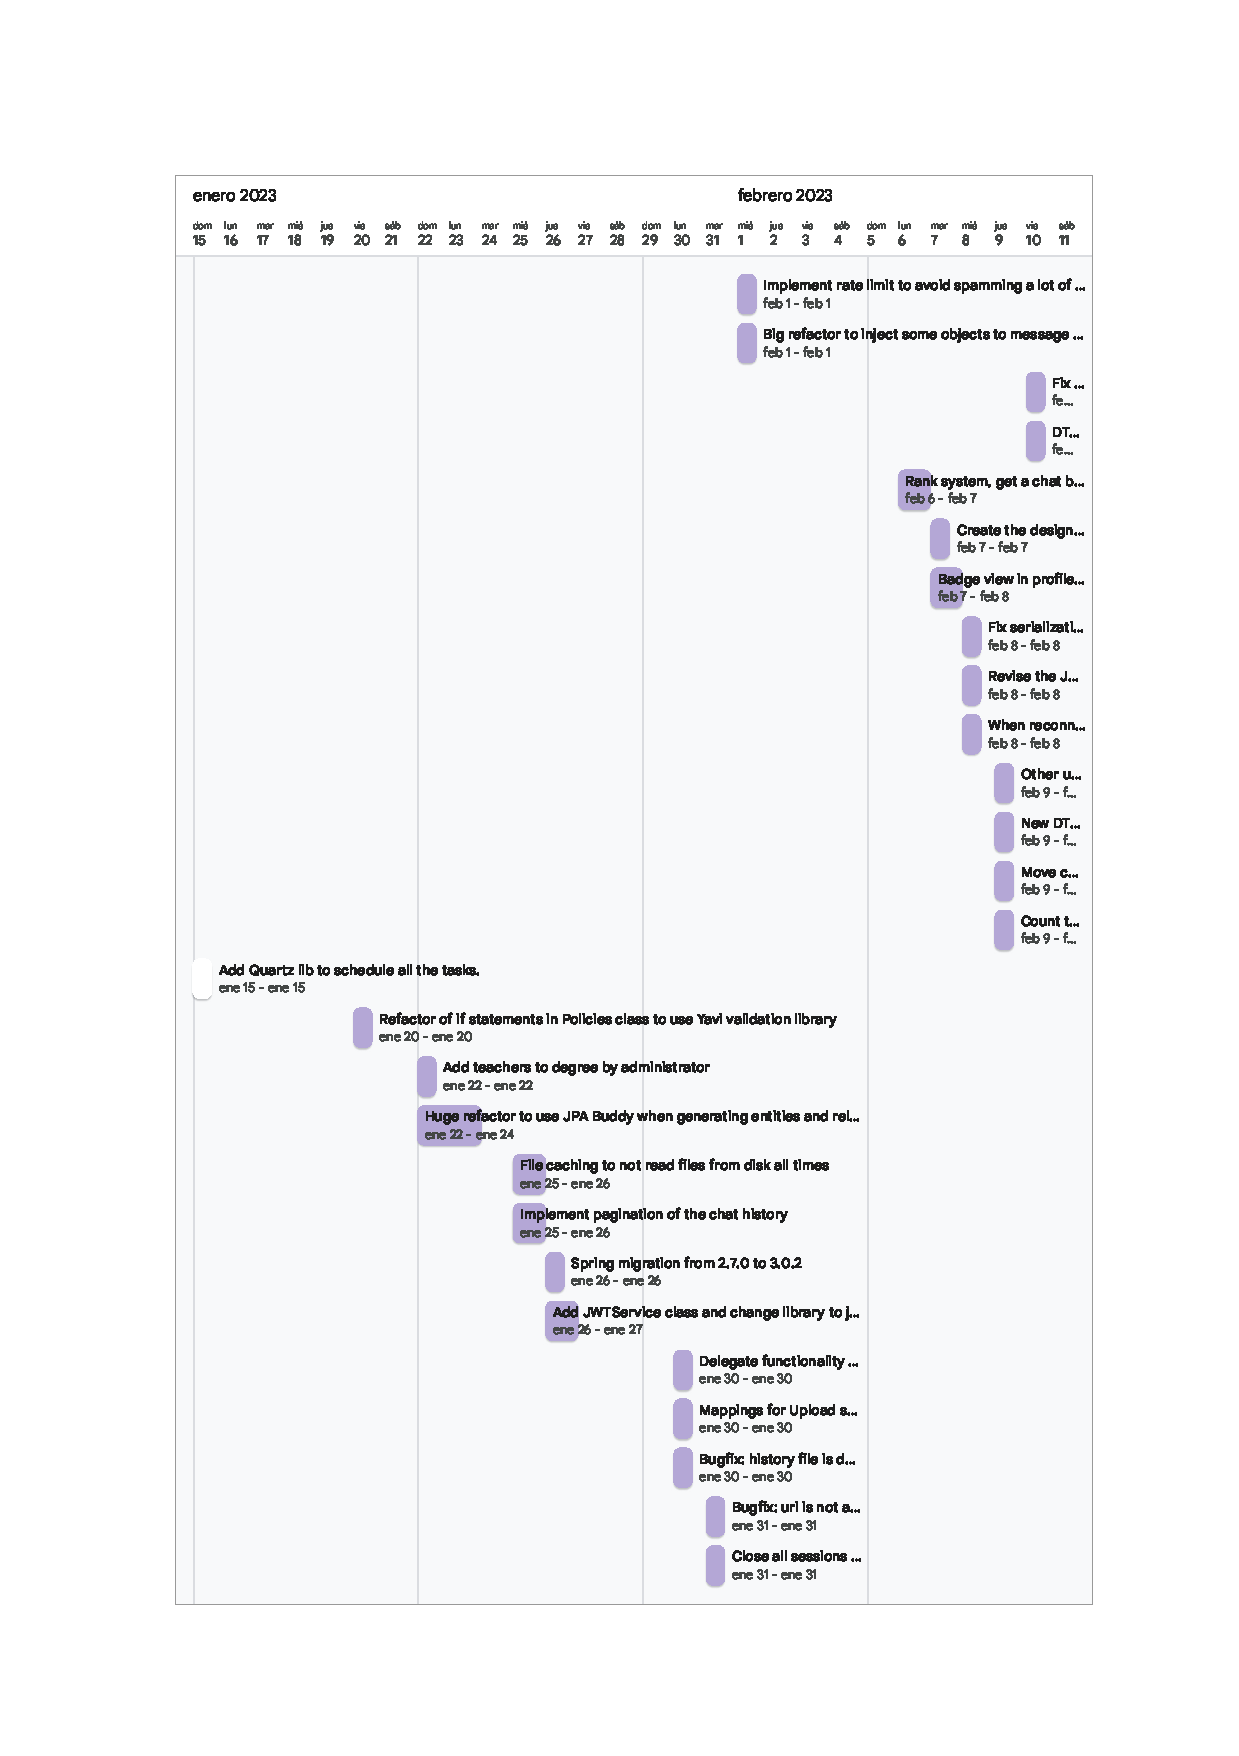
\includepdf[pages=-]{backlog/sprints/Sprint8.pdf}
